\subsection{Measured Temperature Association and Causal Identification}\label{sec:temperature-association}

\subsubsection{Causal Graph for the Temperature Effect}

In uncontrolled observational data, equating a statistical association with a physical temperature effect is risky. We therefore frame the analysis with a structural causal model (SCM)\cite{pearl2009}. Let $D$ and $S$ denote the drug and solvent structures, $T$ the temperature, $Y$ the log-solubility, and $U$ the unrecorded environmental and experimental confounders (measurement protocol, solid-state polymorph transitions, equilibration time, and so on).

The causal directed acyclic graph (DAG) is shown in Figure~\ref{fig:causal-dag}.
\begin{figure}[htbp]
\centering
\begin{tikzpicture}[
  >=Stealth,
  obs/.style={draw, circle, minimum size=0.85cm, inner sep=0pt, font=\small},
  latent/.style={draw, circle, dashed, minimum size=0.85cm, inner sep=0pt, font=\small},
  causal/.style={->, red, very thick},
  arrow/.style={->, gray}
]
\node[obs] (D) at (0,2.0) {$D$};
\node[obs] (S) at (0,0.0) {$S$};
\node[obs] (T) at (2.5,1.0) {$T$};
\node[obs] (Y) at (5.0,1.0) {$Y$};
\node[latent] (U) at (2.5,-1.3) {$U$};
\draw[arrow] (D) -- (T);
\draw[arrow] (S) -- (T);
\draw[arrow] (D) to[out=-20, in=150] (Y);
\draw[arrow] (S) to[out=20, in=-150] (Y);
\draw[arrow] (U) -- (T);
\draw[arrow] (U) -- (Y);
\draw[causal] (T) -- (Y);
\end{tikzpicture}
\caption{Causal DAG for the temperature effect. Solid circles are observed variables, the dashed circle is the unmeasured confounder; the red arrow $T \to Y$ is the target causal path and the grey arrows are backdoor paths.}
\label{fig:causal-dag}
\end{figure}
In this graph the path $T \to Y$ is the causal response of interest, the change in log-solubility when the temperature changes. Two serious backdoor paths exist: the drug and solvent structures correlate with the temperature window chosen, giving the structural backdoor $T \leftarrow (D, S) \to Y$; and experiments at different temperatures may differ in their instrument protocols, giving the environmental backdoor $T \leftarrow U \to Y$.

\subsubsection{Resolving Simpson's Paradox}

To block the structural backdoor $T \leftarrow (D, S) \to Y$, we keep all complete drug--solvent combinations with at least two distinct temperatures: 157 combinations, 73 parents, and 1118 records (median temperature span $27.1^\circ\text{C}$).

On this set, contrasting two regressions exposes the distortion. The pooled ordinary least squares (OLS) yields $\widehat\beta_{\mathrm{pooled}} = -0.00746$ (Figure~\ref{fig:v2-temperature-associations}), a negative correlation that contradicts endothermic dissolution and betrays a Simpson's paradox. The sign flip stems from the correlation between temperature and insolubility in the sample: poorly soluble systems are measured more often at higher temperatures, which manufactures a spurious negative correlation at the pooled level.

Within-combination fixed-effects regression, by contrast, fits
\begin{equation}
Y_{ic} = \alpha_c + \beta_{\mathrm{within}} T_{ic} + \varepsilon_{ic}, \qquad \widehat\beta_{\mathrm{within}} = \frac{\sum_c\sum_i (T_{ic} - \bar T_c)(Y_{ic} - \bar Y_c)}{\sum_c\sum_i (T_{ic} - \bar T_c)^2}.
\end{equation}
De-meaning within each combination removes the structural intercept $\alpha_c$ entirely, blocking all temperature-invariant drug and solvent confounding.

\subsubsection{Within-Group Temperature Slope and Uncertainty}

The estimates appear in Figure~\ref{fig:v2-temperature-associations}. On exactly the same 1118 records, the within-combination fixed-effects slope is
\begin{equation}
\widehat\beta_{\mathrm{within}} = +0.01538.
\end{equation}
That is, each $1^\circ\text{C}$ increase raises the mean log-solubility by 0.01538, a net molar-solubility gain of about 3.6\%.

\begin{figure}[htbp]
\centering
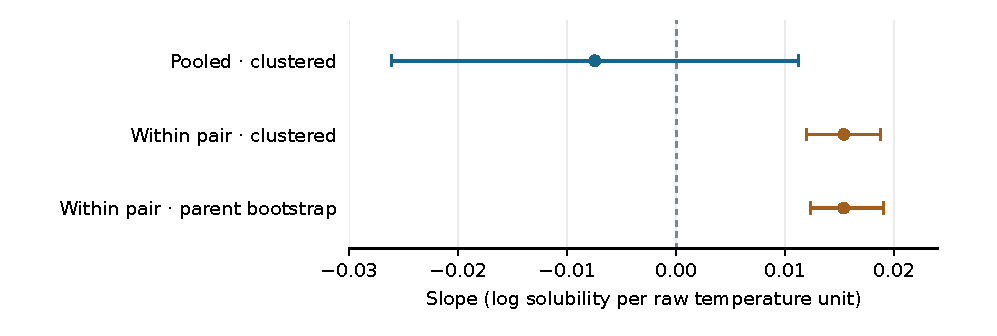
\includegraphics[width=\linewidth]{temperature_associations.pdf}
\caption{Statistical association and causal identification between temperature and measured log-solubility. The first row is the pooled OLS regression; the second and third rows are the within-combination fixed-effects slope and its confidence intervals.}
\label{fig:v2-temperature-associations}
\end{figure}

Three uncertainty analyses back the effect. With parent-clustered robust errors, the 95\% interval is strictly positive, $[0.0121, 0.0186]$; a parent-clustered bootstrap with 2000 resamples gives the percentile interval $[0.01236, 0.01902]$; and a leave-one-parent-out jackknife over the 73 parents keeps the slope within $[0.01424, 0.01599]$. All are positive, so the effect is robust across parents.

\subsubsection{Sensitivity to Unmeasured Confounding}

Fixed effects remove all structural invariants, but a temperature-varying unmeasured confounder $U$ (a polymorph transition or a different measurement time at different temperatures) could in principle still bias the estimate. We therefore apply the Cinelli--Hazlett sensitivity framework\cite{sensitivity2020}. Let $r_T^2$ be the partial $R^2$ of $U$ on $T$ after controlling for the combination effects, and $r_Y^2$ the partial $R^2$ of $U$ on $Y$. Using the omitted-variable-bias identity, we compute the minimal confounding strength needed to drive the adjusted temperature slope to zero (the robustness value). Under the worst-case same-direction bias, the requirement is
\begin{equation}
r_T^2 = r_Y^2 \approx 0.54.
\end{equation}
An unmeasured confounder would have to explain at least 54\% of the residual variance of both temperature and solubility to overturn the positive effect. That degree of co-variation is unlikely for instrument and operational variation in these measurements.

\subsection{Summary}

Taken together, these analyses establish a clear interpretive and causal picture. The ExtraTrees--TabPFN decisions depend mainly on the drug's intrinsic structure and on solute--solvent polarity and hydrogen-bond complementarity, in line with the molecular physicochemical mechanism of dissolution. Within-combination de-meaning resolves the Simpson's paradox in the observational data and pins down a trustworthy positive temperature slope ($+0.01538$), which informs process temperature optimisation. For extrapolation to entirely new parents, the temperature prediction remains a conditional statistical response; in a real crystallisation campaign, the critical points should be checked experimentally under standard operating procedures.
